% !TEX encoding = UTF-8
% !TEX TS-program = pdflatex
% !TEX root = ../tesi.tex
% !TEX spellcheck = it-IT

%**************************************************************
\chapter{Il contesto aziendale}
\label{cap:contesto-aziendale}
%**************************************************************

\section{L'azienda CoffeeStrap inc.}

CoffeeStrap inc\footnote{\url{http://www.coffeestrap.com/}}. è un'azienda \gls{start-up} in ambito web/mobile nata nei primi mesi del 2013 dalla collaborazione di Mahesh Casiraghi e Alessandro Maccagnan, che attualmente ricoprono al suo interno rispettivamente i ruoli di \gls{CEO} e \gls{CTO}. Dal mese di Aprile del 2014 inoltre si è aggiunto al team un ulteriore componente, Milo Ertola, che attualmente ricopre il ruolo di \gls{CPO} e si occupa dello sviluppo web. 

\begin{figure}[htpd]
\centering

\includegraphics[width=\textwidth/2]{../immagini/coffeestrap-logo}
\caption{Logo di CoffeeStrap inc.}  
\end{figure}

La start-up nasce con sede operativa a San Francisco, in cui ha trascorso il suo primo anno di sviluppo, per poi spostarsi all'inizio del 2014 nel cuore Amsterdam, partecipando al programma dell'\gls{acceleratore} Rockstart\footnote{\url{http://www.rockstart.com/accelerator/}}, che fornisce attualmente supporto diretto all'azienda, mettendo a disposizione, oltre alle postazioni di lavoro (è infatti anche \gls{incubatore}), un ambiente fresco e innovativo, circondato da esperti del settore e a stretto e costante contatto con il mondo esterno e con la rete degli investitori. Rockstart possiede al suo interno inoltre un gruppo di \textbf{mentori}, che mettono a disposizione la loro esperienza e le loro capacità, fornendo assistenza diretta in diversi ambiti. Questo tipo di figura è molto importanti in un ambiente di questo tipo, in quanto le aziende, essendo alle origini, hanno bisogno di essere indirizzate nella giusta direzione per poter sviluppare il proprio prodotto in modo efficace e ricevere dunque finanziamenti. La sede operativa contestualmente al mio stage è stata appunto quest'ultima, nella quale ho potuto conoscere il mondo delle start-up ed entrare in contatto con una comunità di sviluppatori, esperti di business e mentori che hanno contribuito alla mia crescita sia professionale che personale.

Rockstart è suddiviso in quattro sezioni principali, ciascuno con il proprio scopo e modalità operative:

\begin{itemize}

\item \textbf{Rockstart accelerator}, che fornisce un programma di accelerazione di 150 giorni, offrendo inoltre un finanziamento iniziale in cambio di una percentuale di quota societaria. Esso si suddivide a sua volta in due sotto-branchie:

\begin{itemize}

\item \textbf{Web e mobile accelerator program}, focalizzato sulle startup in ambito web/mobile. È esattamente in questa branchia in cui l'azienda CoffeeStrap colloca la propria posizione all'interno di Rockstart;

\item \textbf{Smart energy}, che fornisce supporto nelle startup che mettono in correlazione l'\textit{information technology} con il problema del risparmio energetico. Il loro programma differisce leggermente rispetto al precedente.

\end{itemize}

\item \textbf{Rockstart spaces}, che si occupa della gestione degli uffici e degli eventi all'interno di Rockstart. Quest'ultimo ospita infatti al suo interno numerosi eventi nella spaziosa \textbf{ballroom}, molto spesso organizzati da entità al di fuori di Rockstart;

\item \textbf{Rockstart answers}, che organizza eventi mirati a creare una sorta di comunità all'interno di Rockstart nella quale tutti possono confrontarsi tra di loro e

\item \textbf{Rockstart impact}, che fornisce supporto alle start-up nei paesi in via di sviluppo, in particolare in Nepal. 

\end{itemize}

\subsection{Il contesto della start-up}

L'azienda ospitante è una particolare realtà aziendale, l'impresa è nella sua fase iniziale e, come la maggior parte delle start-up, parte con un'idea di riferimento, cercando di rendere profittevole quest'ultima tramite veloci iterazioni sul prodotto. L'incubatore all'interno del quale lavoravo incapsula questo mondo in maniera molto significativa. Sono entrato in un ambiente molto personalizzante, nel quale si è a stretto contatto con il team (essendo quest'ultimo inoltre di piccole dimensioni) e le altre aziende, con le quali si è creata un'implicita rete collaborativa, dalla quale è possibile imparare molto e confrontarsi quotidianamente. Tale collaborazione fornisce valore al prodotto e all'azienda, in quanto permette, oltre ad un importante feedback sulle iterazioni, anche una quotidiana attività di \gls{brainstorming}, che permette di visualizzare i problemi sotto punti di vista differenti e ad arrivare così ad una migliore soluzione.

\section{Il dominio applicativo}

L'idea di CoffeeStrap è quella di fornire un sistema \gls{peer-to-peer} per l'apprendimento di una lingua straniera tramite interazioni con altre persone che parlano quella determinata lingua. L'intento è quello di creare una comunità di utenti che vogliano imparare una lingua e siano allo stesso tempo disposti a fornire supporto ad altri utenti con le lingue cui sono già fluenti. L'interazione può avvenire tramite \textbf{comunicazione testuale}, in cui viene messa a disposizione una vera e propria \textit{chat}, oppure tramite \textbf{comunicazione audio/video}, in cui gli utenti parlano tra di loro nella lingua concordata. Gli utenti hanno la possibilità di iscriversi tramite email o tramite facebook. Il profilo utente è caratterizzato dai seguenti campi:

\begin{itemize}

\item Nome;
\item Cognome;
\item Età (opzionale);
\item Immagine profilo;
\item Città di provenienza;
\item Lingue conosciute;
\item Lingue da imparare.

\end{itemize}

Una volta completato il profilo l'utente inizia a parlare una lingua passando attraverso un flusso:

\begin{itemize}

\item L'utente $X$ seleziona la lingua $Y$ che vuole praticare;
\item Il sistema cerca all'interno della comunità un sottoinsieme $Z$ di persone che parlano la lingua $Y$ (come lingua madre o seconda lingua);
\item Il sistema notifica quest'ultimo, informando gli utenti che l'utente $X$ vuole praticare la lingua $Y$;
\item Gli utenti del sottoinsieme $Z$ decidono se accettare o meno la richiesta dell'utente $X$ di praticare la lingua $Y$;
\item Se l'utente accetta la richiesta allora viene creato un \textbf{match} tra quest'ultimo e l'utente $X$, ed essi iniziano un'interazione.

\end{itemize}

\begin{figure}[htpd]
\centering
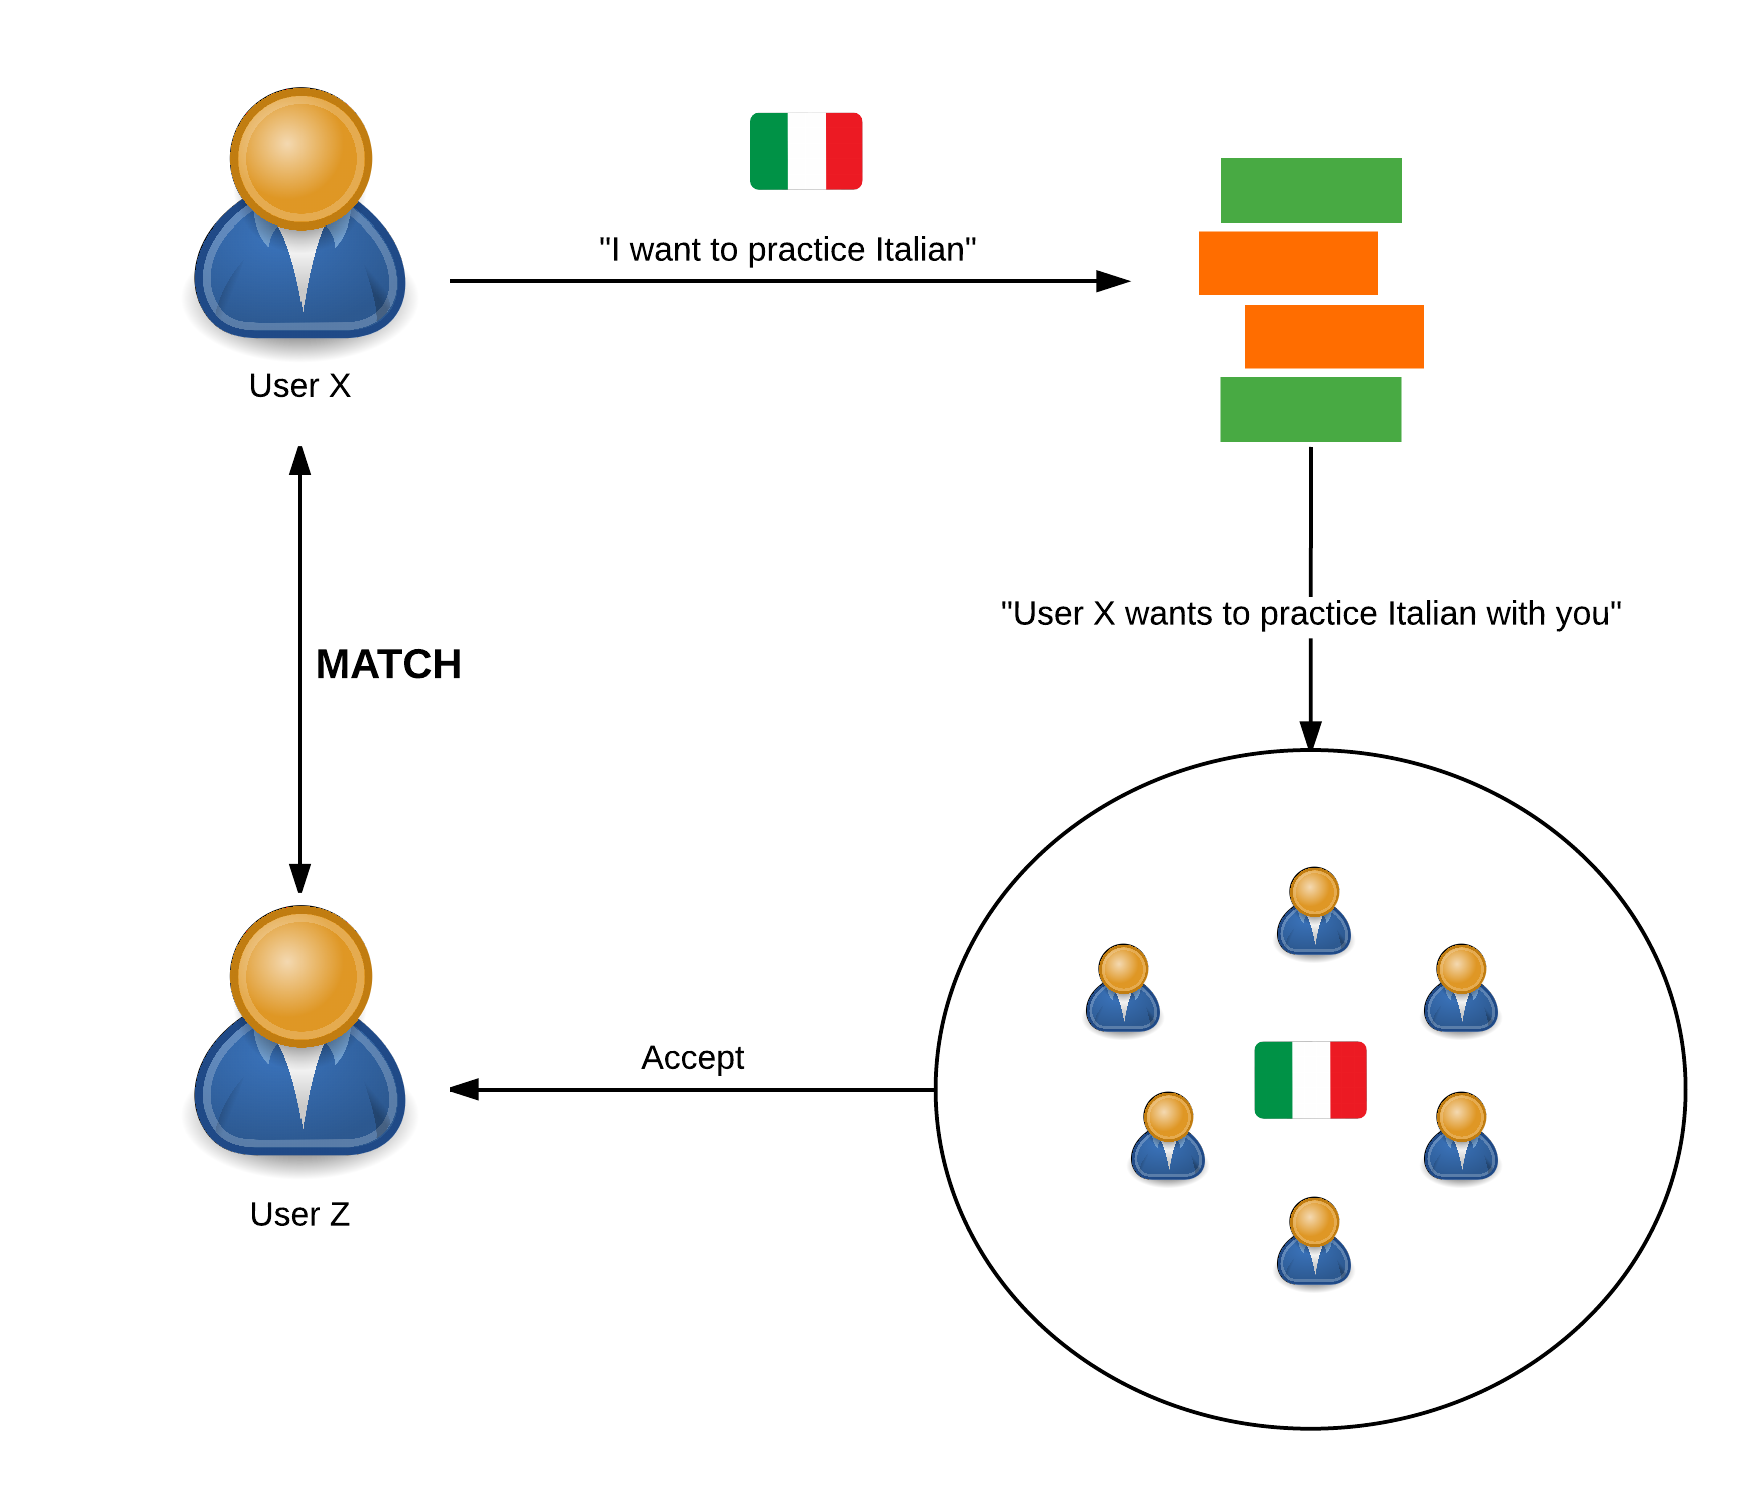
\includegraphics[width=\textwidth]{../immagini/coffeestrap-flow}
\caption{Flusso utente}
\end{figure}

Gli utenti vengono notificati tramite \textbf{notifica email} e, in seguito allo sviluppo dell'applicazione, \textbf{notifica mobile}.

\section{Metodologie e strumenti di sviluppo}

CoffeeStrap adotta la metodologia di sviluppo \textbf{\gls{agile}}. Il particolare contesto entro il quale si trova fa sì che i requisiti cambiano molto spesso e porta dunque quest'ultima a dover iterare molto velocemente sul proprio prodotto, che si trova ancora nella sua fase primordiale e necessita di modifiche e miglioramenti costanti. Proprio a fronte di queste necessità è importante mantenere la massima flessibilità possibile nello sviluppo, motivo per cui questo modello di ciclo di vita è in questo momento il più conveniente in termini di efficienza ed efficacia. In particolare la metodologia adottata è quella \textbf{agile \gls{scrum}}.

Il tipo di iterazione utilizzata è su base settimanale. Una volta a settimana, normalmente il Mercoledì, avviene lo \textbf{scrum meeting}, una riunione della durata di circa due ore nella quale si fissano \textbf{stories} da risolvere nello \textbf{\gls{sprint}} corrente. Una story è un concetto molto simile a quello di \textbf{ticket}, ed è composta dai seguenti campi:

\begin{itemize}

\item \textbf{Titolo};
\item \textbf{Tipologia}, che può assumere i seguenti valori:

	\begin{itemize}

	\item \textbf{Feature}, quando c'è da aggiungere un ``pezzo'' al sistema;
	\item \textbf{Bug}, quando c'è da risolvere una problematica all'interno del sistema;
	\item \textbf{Chore}, quando c'è da eseguire \textit{refactoring} e manutenzione del codice;
	\item \textbf{Release}, sono marcatori di \textit{milestone} che tracciano il progresso del team rispetto agli obiettivi.

	\end{itemize}

\item \textbf{Descrizione}, che fornisce una dettagliata sintesi della story.
\item Una o più \textbf{etichette}, che forniscono un filtro alle stories;
\item \textbf{Complessità}, che è un indice soggettivo di quante risorse sono necessarie per il completamento della story. Questo valore segue la sequenza di Fibonacci e può assumere i valori 1, 2, 5, 8, 13. Se una story ha una complessità superiore a 13 essa dev'essere necessariamente spezzata in due o più sotto-stories. Solamente alle features può essere assegnata complessità, in quanto sono le uniche stories che realmente forniscono un valore al business;
\item \textbf{Richiedente}, che dev'essere unico;
\item Uno o più \textbf{responsabili} (\textit{owners}), che possono coincidere con il richiedente e sono coloro che devono occuparsi direttamente della story;

\end{itemize}

Opzionalmente inoltre è possibile aggiungere alla story dei tasks, in modo da dividere ulteriormente il lavoro. Ciononostante su di essi non vi è alcun controllo, in quanto il loro utilizzo è a discrezione dei responsabili.

\begin{center}
\begin{table}[htpd]
  \begin{tabularx}{\textwidth}{ | c | X |}
    \hline
    \textbf{Titolo} & Login/registrazione con Facebook \\
    \hline
    \textbf{Tipologia} & Feature \\
    \hline
    \textbf{Descrizione} & È necessario interfacciarsi con le API di facebook per Android per poter implementare il sistema di login/registrazione tramite facebook. Una volta ottenuto il token di accesso l'applicazione deve effettuare una chiamata API a CoffeeStrap fornendo quest'ultimo e memorizzando il cookie restituito dalla chiamata. \\
    \hline
    \textbf{Etichette} & \texttt{Mobile} \\
    \hline
    \textbf{Complessità} & 8 \\
    \hline
    \textbf{Richiedente} & Alessandro Maccagnan \\
    \hline
    \textbf{Responsabili} & Luca De Franceschi \\
    \hline
  \end{tabularx}
  \caption{Un esempio di story}
 \end{table}
\end{center}

Ciascuna story è inserita all'interno di una \textbf{board}. Ci sono tre tipologie di board:

\begin{itemize}

\item \textbf{Current}, contenente le stories attive nello sprint corrente;
\item \textbf{Backlog}, contenente la ``coda'' delle stories da attivare;
\item \textbf{Icebox}, contente stories in attesa di approvazione e attivazione. Le stories possono rimanere su questa board per un tempo indeterminato, finché vengono spostate sul backlog o rimosse definitivamente.

\end{itemize} 

A ciascun membro del team vengono assegnate una o più stories, la cui scadenza è lo scrum meeting successivo. A quest'ultimo viene richiesto inoltre di assegnare la complessità a quella story, la quale dovrà essere calcolata secondo criteri derivati dalla propria esperienza di sviluppo. Ogni story dev'essere analizzata, progettata, sviluppata e infine testata. La chiusura della story viene effettuata solamente al seguito di una verifica e validazione da parte del responsabile e del richiedente o, se il richiedente coincide con il responsabile, da un altro membro del team. In generale i responsabili non possono approvare le proprie stories.

Una volta creata la story deve passare attraverso diverse fasi, per questo si parla di \textbf{story workflow}:

\begin{enumerate}

\item La story viene \textbf{creata} e \textbf{definita} (\textit{define and design});
\item I responsabili assegnano loro una \textbf{stima di complessità}, che va generalmente discussa all'interno del team (\textit{estimate});
\item La story viene \textbf{attivata}: da questo momento i responsabili possono procedere allo sviluppo (\textit{start});
\item La story una volta implementata viene \textbf{testata} (\textit{test});
\item Superata la fase di testing la story viene \textbf{ultimata} (\textit{finish});
\item A questo punto i responsabili ``pushano'' il codice sull'ambiente di \textbf{staging} (\textit{deliver});
\item La story viene poi \textbf{accettata} dal richiedente o comunque da una persona esterna al gruppo di responsabili e viene effettuato il pushing sull'ambiente di \textbf{production} (\textit{accept}). Se la story non viene accettata si itera dal punto 4;
\item Infine, se la story è stata accettata avviene il suo \textbf{rilascio}, che coincide con la terminazione del suo ciclo di vita (\textit{release}).

\end{enumerate}

\begin{figure}[htpd]
\centering
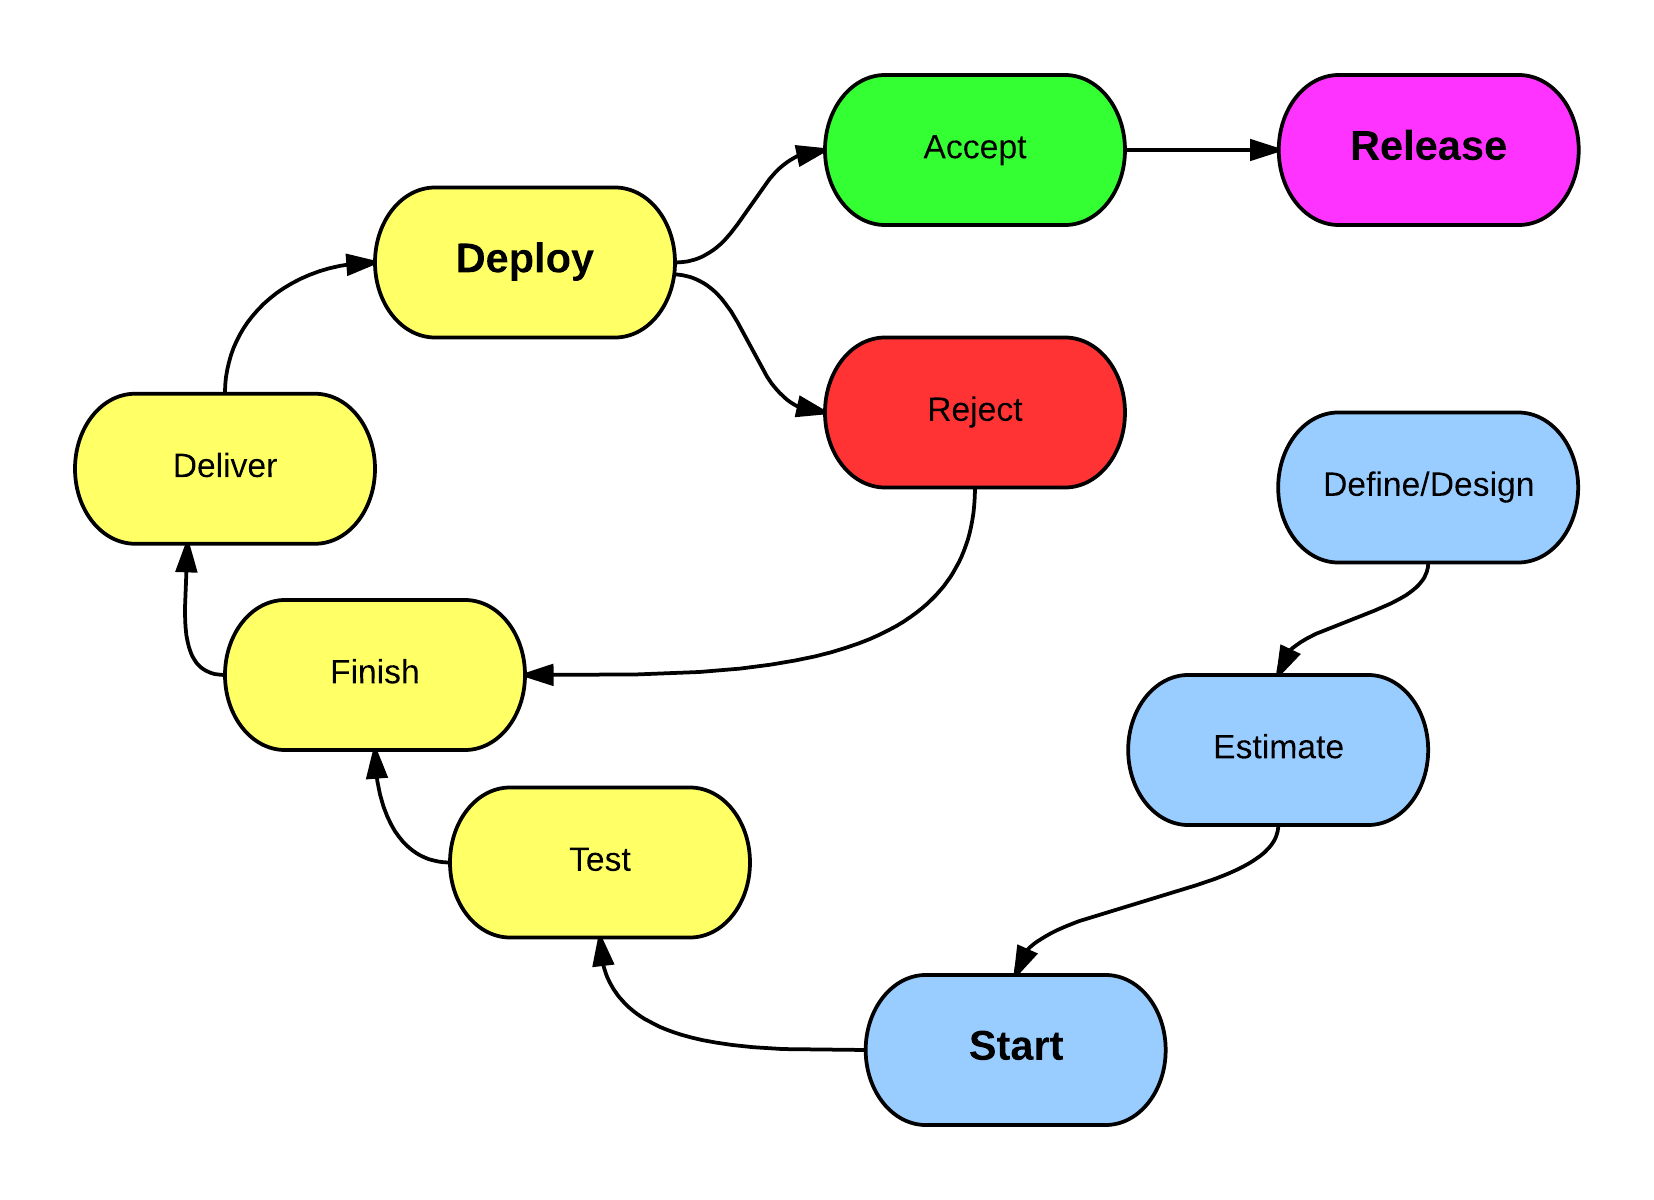
\includegraphics[width=\textwidth]{../immagini/story-workflow}
\caption{Il flusso di una story}
\end{figure}

Alla fine dello sprint viene tracciata la somma delle complessità di tutte le stories assegnate a tutti i membri e che sono state chiuse nello sprint corrente. Tale somma è detta \textbf{velocity}, ed è un indice di efficienza di sviluppo dello sprint, che va confrontato con gli sprint precedenti.

Oltre allo scrum meeting viene instanziato quotidianamente lo \textbf{stand-up meeting}, detto anche \textbf{daily scrum}, nel quale prima dell'inizio della giornata lavorativa si effettua una breve riunione con il team, in cui ciascuno espone quanto fatto nel giorno precedente e ciò che ha in programma di fare nel giorno corrente. Quest'attività è di fondamentale importanza per \textbf{monitorare} il progresso dello sprint e sollevare eventuali difficoltà riscontrate nello svolgimento della story. 

\section{Tecnologie}

\subsection{Back-end}

Il back-end è composto da un server scritto tramite il framework \gls{Node.js}. Questa scelta è dovuta alla grande potenza e scalabilità di quest'ultimo, oltre al fatto che si tratta di un linguaggio di programmazione all'avanguardia la cui comunità è in forte espansione. Inoltre tramite \textbf{npm}, gestore di pacchetti per Node.js, è possibile attingere ad una vasta quantità di librerie.

Il server fornisce tutta una serie completa di \textbf{\gls{API} \gls{REST}ful} accessibili dall'esterno, alcune delle quali richiedono autenticazione. Ciò permette a tutti i client che si interfacciano con esso, in particolare l'applicazione web e l'applicazione mobile, di poter comunicare con esso in modo semplice e lineare, dovendo riferirsi solamente alle specifiche di queste ultime ed utilizzando una libreria per la gestione delle chiamate API. 

\begin{figure}[htpd]
\centering

\includegraphics[width=\textwidth/2]{../immagini/node-js-logo}
\caption{Logo di Node.js}
\end{figure}

Parallelamente al server è stato instanziato un servizio di \textbf{pushing} fornito da \textbf{firebase}, un \textbf{\gls{Cloud Service Provider}} utilizzato per il sistema di notifiche e per fornire un punto d'accesso centralizzato dal quale i diversi componenti (intesi come componenti software) possono comunicare. Firebase fornisce infatti un \textbf{database in tempo reale}, con il quale è possibile interagire e ``\textit{mettersi in ascolto}'' degli eventi su di esso. Esso fornisce un'API pubblica per diversi stack tecnologici e piattaforme.

\begin{figure}[htpd]
\centering

\includegraphics[width=\textwidth/2]{../immagini/firebase-logo}
\caption{Logo di Firebase}
\end{figure}

\subsection{Front-end}

Il front-end è composto da un'applicazione web scritta con \textbf{\gls{Angular.js}} e \textbf{\gls{HTML5}}, utilizzando il framework CSS \textbf{\gls{Bootstrap}}. Tramite Angular.js è possibile interfacciarsi alle API fornite dal back-end in maniera molto efficiente e popolare dunque le pagine in base alle risposte provenienti da esso. Inoltre, analogamente a npm, per lo sviluppo di applicazioni con Angular.js è disponibile \textbf{bower}, gestore di pacchetti per quest'ultimo.

\begin{figure}[htpd]
\centering

\includegraphics[width=\textwidth/2]{../immagini/angular-js-logo}
\caption{Logo di Angular.js}
\end{figure}

\subsection{Database}

CoffeeStrap utilizza \textbf{\gls{MongoDB}} come database documentale di riferimento. Questa scelta è dovuta alla grande flessibilità offerta dai database di questo tipo, oltre al fatto che negli ultimi mesi è divenuto molto popolare nella comunità di sviluppatori e presenta prestazioni notevoli. 

Dal momento che i requisiti cambiano molto rapidamente è necessario avvalersi di strumenti che siano il più flessibili possibili ai cambiamenti, e MongoDB risponde perfettamente a questo tipo di esigenza. Inoltre MongoDB presenta un facile approccio al suo utilizzo sia per l'utilizzo da parte dello sviluppatore che in termini di scalabilità.

\begin{figure}[htpd]
\centering

\includegraphics[width=\textwidth/2]{../immagini/mongo-db-logo}
\caption{Logo di MongoDB}
\end{figure}

\subsection{Ambienti di sviluppo}

All'interno dell'azienda si delineano principalmente due ambienti di sviluppo:

\begin{itemize}

\item \textbf{Production}, all'interno del quale risiedono le versioni ufficiali del codice esposte pubblicamente agli utenti;

\item \textbf{Staging}, un ambiente riservato esclusivamente al team e che rappresenta una sorta di ``cantiere'', nel quale risiede una versione del codice ancora da verificare, che può quindi essere testata liberamente e non crea danni verso l'esterno.

\end{itemize}

Ciascun ambiente è caratterizzato dalla propria configurazione, possiede il proprio server e il proprio database ed è agnostico rispetto all'altro.

Occasionalmente è inoltre uso comune instanziare un ambiente ausiliario di sviluppo, per circostanze particolari che necessitano di una configurazione diversa. Solitamente sono ambienti ``\textit{usa e getta}'', che nascono da esigenze particolare e vengono rimossi alla fine del loro utilizzo.

\subsection{Versionamento}

Come strumento di controllo versione del codice sorgente l'azienda utilizza \textbf{\gls{Git}}, utilizzando \textbf{Bitbucket} come servizio di hosting. I motivi che hanno spinto all'utilizzo di Git in luogo di altri sistemi di versionamento sono i seguenti:

\begin{itemize}

\item \textbf{Disponibilità}: ciascun sviluppatore ha una copia locale dell'intero repository ed effettua \textit{\gls{commit}} in locale, potendo dunque lavorare anche in assenza di connessione;

\item \textbf{Semplicità}: oltre ad essere veloce Git permette con facilità la creazione di \textit{branch} e successivi \textit{\gls{merge}}. L'utilizzo di questi ultimi è fondamentale per poter soddisfare il punto seguente:

\item \textbf{Utilizzo di Gitflow}: questo \textbf{workflow} definisce uno stretto modello di \textit{branching} che ruota intorno al progetto. Ciò non aggiunge nuovi concetti o strumenti a Git, ma piuttosto assegna ruoli specifici ai diversi rami. Un approfondimento di questa metodologia è raccolta nell'appendice A.

\end{itemize}

\begin{figure}[htpd]
\centering

\includegraphics[width=\textwidth/2]{../immagini/git-logo}
\caption{Logo di Git}
\end{figure}

\section{Clientela di riferimento}

CoffeeStrap non ha ancora acquisito finanziamenti da parte di investitori e non presenta associazioni con altre aziende o entità, motivo per cui essi devono rispondere unicamente agli \textbf{utenti finali} del prodotto. Questi ultimi sono persone reali provenienti da ogni parte del mondo, che mettono a disposizione le proprie competenze linguistiche e vogliono allo stesso tempo imparare una lingua straniera entrando in contatto con altri utenti. L'intera struttura di CoffeeStrap si basa su questa \textbf{rete sociale}, composta da un insieme eterogeneo di persone che espongono il proprio profilo all'esterno. È possibile immaginare CoffeeStrap come un vero e proprio \textit{social network} il cui scopo è l'apprendimento linguistico.

\begin{figure}[htpd]
\centering
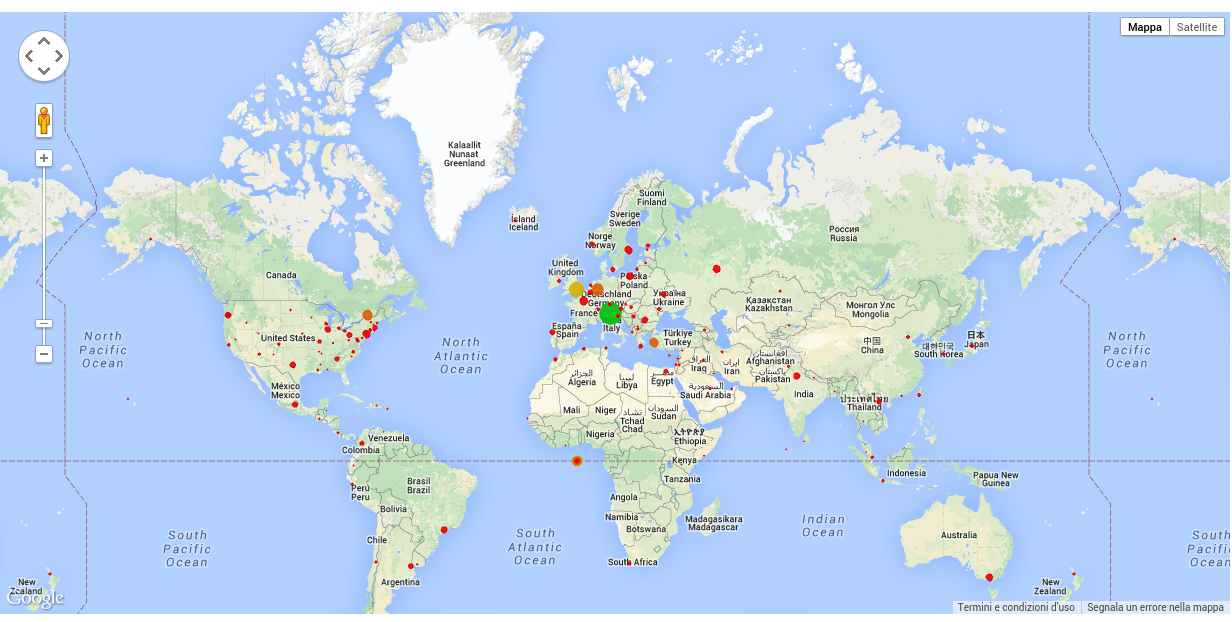
\includegraphics[width=\textwidth]{../immagini/user-distribution}
\caption{Distribuzione degli utenti di CoffeeStrap nel mondo aggiornata a Dicembre 2014}
\end{figure}